\documentclass[11pt,a4paper]{article}

\usepackage[twoside,a4paper,hmarginratio=3:2,vmarginratio=1:1,bmargin=2.54cm]{
geometry}                % See geometry.pdf to learn the layout options. There are lots.
\geometry{a4paper}                   % ... or a4paper or a5paper or ... 
%\geometry{landscape}                % Activate for for rotated page geometry
%\usepackage[parfill]{parskip}    % Activate to begin paragraphs with an empty line rather than an inden

\usepackage{graphicx}
\usepackage{graphics}
\usepackage{amssymb}
\usepackage{amsmath}
\usepackage{epstopdf}
\usepackage{longtable}
\usepackage{lscape}
%\usepackage{savepapr}
\usepackage{fancyhdr}
\usepackage{fancybox}
\usepackage{indentfirst}
\usepackage{ifthen}
\usepackage{comment}
\usepackage{flafter}
%%%\usepackage{reenumi}
\usepackage{bibentry}
%\usepackage{hyperref}

\usepackage[latin1]{inputenc}
\usepackage{amsmath}
\usepackage{amsfonts}
%\usepackage{makeidx}
\usepackage{bm}
\usepackage{multicol}
\usepackage{color}

\newcommand{\dif}{\mathsf{d}}

%%---------------------------------------------------------------  DJS Definitions 
\def\ffrac#1#2{\leavevmode\kern.1em
\raise.5ex\hbox{\the\scriptfont0 #1}\kern-.1em
/\kern-.15em\lower.25ex\hbox{\the\scriptfont0 #2}}
\def\half{\frac{1}{2}}
\def\hhalf{\ffrac{1}{2}}
\def\bA{\mathbf{A}}
\def\bB{\mathbf{B}}
\def\bC{\mathbf{C}}
\def\bD{\mathbf{D}}
\def\bI{\mathbf{I}}
\def\bP{\mathbf{P}}
\def\bX{\mathbf{X}}
\def\tough{$\!\!\!{}^\star\>$}
\newcommand{\R}{{\mathbb{R}}}


%% Change this boolean to true to compile solutions.
\newboolean{mynotes}
\setboolean{mynotes}{true}

%\setboolean{mynotes}{true}

%%---------------------------------------------------------------------------------------
\begin{document}

\begin{center} 
{\bf Maths Problems for  CHEN10072 \\
\ifthenelse{\boolean{mynotes}}{(With solutions) \\}

 Bill Lionheart
}
\end{center}
\hrule
\smallskip



%%---------------------------------------------------------------------------------------

\section*{Week 7}



%Numerical solution of a scalar nonlinear ODE. Exercises will show that 
%explicit approximation is easy and that implicit approximation leads to 
%a nonlinear equation to be solved at every time step.
 
{\bf Summary of forward Euler}

To solve $$
{\dif y\over \dif t} = f(y,t),\quad y(t_0)=y_0
$$
numerically we choose a step length $h>0$ and then calculate
\begin{eqnarray*}
y_1 &=& y_0 + h f(y_0,t_0),\, t_1=t_0 +h \\
y_2 &=& y_1 + h f(y_1,t_1),\, t_2=t_1 +h \\
y_3 &=& y_2 + h f(y_2,t_2),\, t_3=t_2 +h \\
\mbox{etc.}
\end{eqnarray*}
in which case $y_i$ is an approximation  to $y(t_i)$ at each step. The approximation should get more accurate as $h$ gets smaller. The error at each step will get worse if $\dif^2 y/ \dif t^2$ is large and these errors can build up for longer time intervals.
 
\begin{enumerate}
 \item \label{qdjsode1}
 We would like to  to solve the differential equation
$$
{\dif y\over \dif t} = -10(t-1)y
$$
with the given  initial condition:
$y(0)=e^{-5}$. 
{A reference  solution to this problem can  be
plotted in MATLAB  by  typing the command sequence}  
\begin{verbatim} tt=0:0.01:2; ex=exp(-5*(tt-1).^2);plot(tt,ex,'-k')}
\end{verbatim}
\begin{enumerate}
\item 
Find the analytic solution $y(t)$, and evaluate it at\\
$t=0.2,0.4, 0.6, 0.8, 1.0, 1.2$ and  $1.4$.


\item
Compute the forward Euler solution by  taking {\it seven} steps of the method
with a step length of $h=0.2$. (You will need a calculator to do this.)
Generate a table which
compare the analytic solution with the numerical solution. At which
time $t$ do you find the biggest error ?

\item
Compute a more accurate  forward Euler solution  by  taking  four steps with
a  much smaller step length of $h=0.05$. Compare this solution
with the exact solution  $y(0.2)$ and compare the accuracy of this  solution
with the first time step result  obtained in (b).
\end{enumerate}

Note that  this differential equation  is not as benign as
it looks; if one wants to solve it over a long time interval,
sophisticated numerical methods (like those that are built into MATLAB)
 are needed. A simple example of a sophisticated method is
 the implicit Euler method which will be discussed in the lectures. 
\end{enumerate}

 \ifthenelse{\boolean{mynotes}}{
{\bf Solution}

\noindent\hrulefill

\begin{enumerate}
\item Analytical solution is $y(t)=\exp(-5(t-1)^2)$

Plot of exact solution
\begin{center}
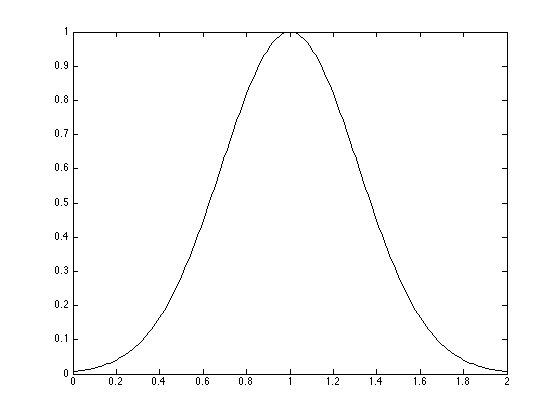
\includegraphics[scale=0.3]{week07ans1.png}
\end{center}
 
\begin{center}
$h=0.2$

\begin{tabular}{|c|c|c|c|c|c|c|c|c|c|}
\hline
$t$ & 0  &  0.2000  &  0.4000  &  0.6000 &   0.8000 &   1.0000 &
   1.2000  &  1.4000 \\
  \hline
$y$ & 0.0067  &  0.0408  &  0.1653  &  0.4493 &   0.8187  &  1.0000
  &  0.8187 &   0.4493 \\
\hline
$y_i$ & 0.0067  &   0.0202 &   0.0526  &  0.1156  &  0.2081  &  0.2914
&   0.2914  &  0.1748 \\
  \hline
 \end{tabular}
\end{center}


\begin{center}
$h=0.05$

\begin{tabular}{|c|c|c|c|c|c|}
\hline
$t$ &  0  &  0.0500  &  0.1000  &  0.1500  &  0.2000 \\
  \hline
$y$  & 0.0067  &  0.0110  &  0.0174  &  0.0270 &   0.0408 \\
\hline
$y_i$ & 0.0067  &  0.0101  &  0.0152 &   0.0227  &  0.0341 \\
  \hline
 \end{tabular}
\end{center}

\end{enumerate}

}{}% 
 
\vfill\eject
%%---------------------------------------------------------------------------------------


%%---------------------------------------------------------------------------------------

\end{document}
